\chapter{Introduction}

Formal verification has emerged as the gold standard
for ensuring correctness in computer systems,
offering mathematical proofs that provide
unparalleled assurances compared to conventional testing.
However, formal verification faces significant challenges
when applied to large-scale and heterogeneous systems.
Such systems combine diverse operational paradigms,
complex stateful interactions,
and multiple abstraction levels,
creating substantial obstacles
for traditional verification approaches.

Traditional verification frameworks
rely on simplified, monolithic operational semantics models.
While mathematically tractable,
these models have significant limitations
for complex, real-world systems.
They assume closed, static environments
that cannot adequately model
the dynamic interactions characteristic of modern computing systems.
Moreover, monolithic models
lack the flexibility to integrate
multiple verification methodologies and tools,
limiting their practical scalability.

\section{Verification Challenges in Complex Systems}

\subsection{Motivating Examples}

Software development typically follows two broad programming patterns.
The first pattern focuses on implementing data structures or algorithms
as reusable libraries for other programs.
For this style of programming,
the bounded queue example from \citet{rbgs-cal} is adopted,
whose source code is shown in Fig.~\ref{fig:bq-code}.
The queue is built in two layers:
$\kw{rb.c}$ exposes a ring buffer
backed by an array along with two counters
that wrap around on overflow or underflow,
while $\kw{bq.c}$ builds on this abstraction
to provide queue operations.

\begin{figure}[t!]
  \center
  \hspace{-5.5em}
  \begin{subfigure}{0.6\textwidth}
\begin{minted}[fontsize=\small,frame=single,numbersep=0.3em]{c}
static int c1, c2;
static V buf[N];

int inc1() { int i = c1++; c1 %= N; return i; }
int inc2() { int i = c2++; c2 %= N; return i; }
V get(int i) { return buf[i]; }
void set(int i, V val) { buf[i] = val; }
\end{minted}
    \vspace{-1em}
    \subcaption{The translation unit $\kw{rb.c}$}
    \label{fig:rb}
  \end{subfigure}
  \hspace{0.5em}
  \begin{subfigure}{0.48\textwidth}
\begin{minted}[fontsize=\small,frame=single,numbersep=0.3em]{c}
extern int inc1(void);
extern int inc2(void);
extern V get(int i);
extern void set(int i, V val);

void enq(V val) { set(inc2(), val); }
V deq() { return get(inc1()); }
\end{minted}
    \vspace{-1em}
    \subcaption{The translation unit $\kw{bq.c}$}
    \label{fig:bq}
  \end{subfigure}
  \hspace{-5.5em}
  \caption{Running example, adapted from \citet{rbgs-cal}.
    The component $\kw{rb.c}$
    implements a ring buffer of capacity $N$
    by encapsulating an array
    and two counters. It is used by %the component
    $\kw{bq.c}$ to implement a
  bounded queue.}
  \label{fig:bq-code}
  %\caption{The state of a ring buffer,
  %  made of two counters and a fixed-size array,
  %  is encapsulated behind a simple interface.}
  %\label{fig:rb}
  %\caption{This component relies on the ring buffer primitives
  %  provided in Fig.~\ref{fig:rb} to implement a bounded-size queue.}
  %\label{fig:bq}
\end{figure}


The second pattern centers on executable programs
that are algorithmically simple
but interact extensively with their external environment.
A representative example is shown in Fig.~\ref{fig:readwritehello},
where two programs share a common C library
and are designed to work together.
The 32-bit x86 assembly program $\kw{secret.s}$ produces an encoded message,
which is then passed through a pipe to $\kw{decode.c}$ for decoding.
Unlike the bounded queue,
the difficulty here lies not in the data structure itself
but in capturing and verifying
the correctness of rich external interactions across heterogeneous components.

\begin{figure} % fig:readwritehello {{{
  \centering
  \begin{minipage}{0.39\textwidth}
      %\begin{lstlisting}[title={secret.c}]
      %#include <unistd.h>
      %char msg[] = "uryyb, jbeyq!\n";
      %int main()
      %{
      %        write(1, msg, sizeof msg - 1);
      %        return 0;
      %}
      %\end{lstlisting}
    \begin{center}
      secret.s
    \end{center}
    \vspace{-1.5em}
      \begin{minted}[fontsize=\small,frame=single,numbersep=0.3em]{gas}
.globl main
main: pushl $13
      pushl $msg
      call rot13
      pushl $1
      call write
      addl $12, %esp
      movl $0, %eax
      ret
.data
msg:  .string "hello, world!\n"
      \end{minted}
    \vspace{-1em}
      \begin{minted}[fontsize=\small,frame=single,numbersep=0.3em]{bash}
$ cc -o secret secret.s rot13.c
$ ./secret
uryyb, jbeyq!
$ cc -o decode decode.c rot13.c
$ ./secret | ./decode
hello, world!
  \end{minted}
  \end{minipage}
  \hspace{0.8em}
  \begin{minipage}{.57\textwidth}
    \begin{center}
      rot13.c
    \end{center}
    \vspace{-1.5em}
      \begin{minted}[fontsize=\small,frame=single,numbersep=0.3em]{c}
void rot13(char *buf, int len) {
  for (int i = 0; i < len; i++)
    if ('a' <= buf[i] && buf[i] <= 'z')
      buf[i] = (buf[i] - 'a' + 13) % 26 + 'a';
}
      \end{minted}
    \vspace{0.4em}
    \begin{center}
      decode.c
    \end{center}
    \vspace{-1.5em}
      \begin{minted}[fontsize=\small,frame=single,numbersep=0.3em]{c}
#include <unistd.h>
extern void rot13(char *, int);
int main() {
  char buf[100];
  int n = read(0, buf, sizeof buf);
  rot13(buf, n);
  write(1, buf, n);
  return 0;
}
      \end{minted}
  \end{minipage}
  \caption{Two programs which use a common library
    are compiled and made to
  interact through a pipe.}
  \label{fig:readwritehello}
\end{figure}

\subsection{Core Verification Challenges}

These examples illustrate the core challenges
that effective verification frameworks must address
for real-world, large-scale systems:

\begin{challenge}
  \label{challenge:abstraction}
  \textbf{Supporting Multiple Levels of Abstraction.}
  Large-scale systems require reasoning
  across multiple abstraction levels,
  each governed by different mathematical frameworks.
  The challenge lies in coherently connecting
  these diverse perspectives.
  For instance,
  microprocessor circuit algebra
  differs fundamentally from
  assembly language operational semantics,
  which in turn differs from
  operating system abstractions
  and high-level programming language semantics.
  Functional specification languages
  provide clean, abstract behavioral views
  precisely because they avoid low-level operational details.

  This challenge applies beyond entire systems
  to individual data structures.
  Complex structures like maps, queues, or trees
  are typically specified functionally in terms of mathematical sets or relations
  but implemented through intricate low-level memory manipulations.
  Data abstraction exemplifies the broader challenge:
  coherently managing relationships
  between multiple views of the same system
  at different abstraction levels.

  Concretely,
  in the bounded queue example,
  the buffer can be specified abstractly
  as a function from integers to values,
  rather than as an array in the C memory model.
  Likewise, the queue itself is naturally described
  as a sequence of values,
  independent of the details of its implementation.
  Handling these different views coherently---whether across entire systems
  or within a single data structure---is essential for scalable and trustworthy verification.

\end{challenge}

\begin{challenge}
  \label{challenge:interaction}
  \textbf{Reasoning in Open Context.}
  Complex programs rarely execute in isolation.
  They interact with other components, libraries,
  or even entirely separate processes,
  and these interactions cannot always be anticipated
  in advance.
  For a verification framework to be realistic and scalable,
  it must support reasoning about program behavior
  in such open contexts%
  ---without relying on the closed-world assumption
  that all possible interactions are fixed
  and known ahead of time.
  Fundamentally, closed-world reasoning requires
  the behavior of external modules to be fixed upfront,
  while open-world reasoning requires only their signatures
  to be fixed,
  allowing the actual behavior to vary
  as long as it respects the interface contract.

  To understand this limitation,
  consider how traditional program semantics handle the bounded queue example.
  Under the closed-world assumption,
  the behavior of \kw{bq.c} remains unclear
  without having the underlying ring buffer functions provided in advance.
  This creates two unsatisfactory options.
  First, one could verify \kw{bq.c} together with
  \kw{rb.c}'s concrete implementation,
  but this approach obviously lacks modularity.
  The second option is to provide the behavior through
  a fixed specification for the ring buffer, say \kw{Spec}$_\kw{rb}$.
  While this seems more modular at first,
  it requires the specification to be completely fixed upfront
  and forces us to choose a particular data representation.
  Once committed to \kw{Spec}$_\kw{rb}$,
  the verification becomes locked into that specific way of thinking
  about the ring buffer's state and operations,
  preventing later substitution of different implementations
  or reasoning about the queue's behavior
  in contexts where the ring buffer might behave differently.

  In contrast, open-world reasoning would allow
  the bounded queue's correctness to be verified
  without presuming how the environment will use it.
  Similarly, when the queue invokes the underlying ring buffer,
  the framework must not hard-code assumptions
  about how the buffer will respond;
  rather, the framework must allow
  the queue's behavior to be modeled
  independently of its precise context of use.
  Reasoning in this way
  ensures that properties established
  for the queue remain valid no matter where, or how,
  it is deployed.

  The same challenge appears
  in the example of two programs communicating through a pipe.
  Each program is simple on its own,
  but their joint behavior
  depends on a dynamic, asynchronous exchange of data.
  Here too,
  verification cannot assume a fixed pattern of interaction.
  Instead,
  it must treat each program as an open component,
  reasoning about its behavior abstractly
  in terms of the inputs
  it may receive and the outputs it may produce.

  In short,
  the difficulty lies not only in proving
  that individual components behave correctly,
  but also in ensuring that
  such proofs remain robust
  when those components are placed
  into unpredictable or evolving environments.
  Supporting this style of open-world reasoning%
  ---where correctness is preserved under arbitrary contexts
  and interactions---is a central challenge
  addressed by this work.

\end{challenge}

\begin{challenge}
  \label{challenge:encapsulation}
  \textbf{State Encapsulation.}
  In complex systems,
  interactions between stateful components
  can cause unintended interference.
  Scalable verification requires
  rigorous state partitioning and encapsulation
  to ensure modular correctness proofs remain valid
  despite dynamic component interactions.

  State encapsulation provides exactly this safeguard.
  By restricting all or part of a component's internal state
  from being accessed directly by its environment,
  it guarantees that
  the state can only be influenced
  through the component's well-defined interface.
  A concrete example is the bounded queue implementation:
  the underlying ring buffer maintains its data in an array
  along with counters for indexing,
  but these internal details should remain hidden.
  The interface of the ring buffer exposes only operations
  such as get and set,
  and the queue itself in turn exposes only its abstract operators
  without revealing its internal representation.
  This disciplined boundary ensures that clients of the queue
  cannot tamper with the ring buffer's internal state,
  and the queue cannot depend on how the ring buffer itself is implemented,
  beyond its interface contract.

  Such encapsulation not only prevents accidental interference
  but also enforces a disciplined boundary of interaction,
  allowing proofs about one component
  to remain stable regardless of the behaviors of others.
  In this way,
  encapsulation strengthens modular reasoning
  and supports the scalable verification of complex systems.

\end{challenge}

\begin{challenge}
  \label{challenge:compilation}
  \textbf{Certified Compilation.}
  Verifying high-level source code alone is insufficient
  because compilation itself can introduce errors.
  End-to-end correctness requires frameworks
  that integrate with certified compilers,
  extending correctness guarantees
  from high-level specifications to machine-executable binaries.

  Certified compilers such as CompCert
  address part of this challenge
  by proving the correctness
  of the compilation process.
  However, ensuring end-to-end correctness
  requires the verification framework
  to seamlessly integrate with this correctness proof.
  Only then can guarantees obtained
  at the source-level components be reliably
  transferred to the generated target program.

  Additionally,
  this integration requires accurately modeling
  how compiled programs transition into executable entities.
  Crucially, for a proof artifact to be truly end-to-end,
  the framework must also model
  the behavior of the compiled assembly programs themselves.
  Capturing these low-level details,
  together with all relevant aspects of
  runtime behavior,
  ensures that the reasoning chain---from high-level specification
  through compiler transformations to final execution---remains unbroken.
  Without this,
  gaps can arise between source-level proofs
  and target-level execution,
  undermining the entire verification effort.
  Bridging this gap is therefore critical.

\end{challenge}

\begin{challenge}
  \label{challenge:multi-language}
  \textbf{Handling Heterogeneous Components.}

  Real-world systems are often heterogeneous,
  combining components written in different programming languages,
  from low-level assembly routines to high-level,
  expressive source code.
  An effective verification framework
  must therefore provide a unified way
  to reason across this spectrum,
  enabling correctness guarantees
  to span both abstract specifications
  and highly optimized machine-level implementations.

  This heterogeneity is not just a matter of convenience
  but of necessity.
  Performance-critical software%
  ---such as operating systems,
  cryptographic libraries,
  or multimedia codecs%
  ---frequently implements their hot paths
  in hand-written assembly
  to maximize performance
  through hardware-specific optimizations.
  For instance,
  cryptographic primitives
  like AES or SHA are often coded
  in assembly to leverage specialized CPU instructions,
  while the surrounding protocol logic
  remains in C or higher-level languages.
  Similarly, real-time systems
  such as network drivers or signal-processing routines
  may utilize assembly for performance-critical sections,
  while delegating control flow and system integration
  to higher-level code.

  The motivating example,
  shown in Figure \ref{fig:readwritehello},
  illustrates this phenomenon directly:
  the component $\kw{secret.s}$ is implemented in x86 assembly to encode a message,
  while the companion program $\kw{decode.c}$---written in C---deciphers it.
  Moreover, the pipe connecting them can itself be viewed as a heterogeneous component,
  since its semantics is defined neither in C nor assembly
  but rather through operating system abstractions.
  Although each component is algorithmically simple,
  their correctness hinges on coherent cross-language reasoning
  about how the two interact through this heterogeneous communication mechanism.

  A verification framework
  that cannot bridge this gap risks
  leaving its most critical
  and performance-sensitive components
  outside the scope of formal guarantees.
  By contrast,
  a robust framework must treat assembly
  and high-level languages
  as part of a single, coherent reasoning space,
  allowing correctness proofs
  to follow programs seamlessly across abstraction levels.

\end{challenge}

\section{Insufficient Existing Approaches}
\label{sec:intro:litreview}

Substantial research has sought to
address the challenges outlined above.
The key to formal verification
is the underlying semantic model that defines
how program behavior is represented and reasoned about.
This section reviews existing approaches
according to their choice of semantic model,
examining how each partially addresses
the verification challenges,
highlighting their contributions and limitations.

\subsection{Operational Semantics}

Operational semantics is the most commonly used approach
because it is intuitive and amenable to reasoning.
Programs are modeled through state transitions
that directly correspond to execution steps,
making the semantic model easy to understand and manipulate.

% Existing work has been conducted
% along the following lines.
% First,
% verification frameworks
% have been built on top of CompCert
% so that an end-to-end
% correctness proof can be delivered,
% thereby solving challenge (c).
% Second,
% a series of work
% have extended CompCert to support
% more advanced programming paradigms,
% including enabling compositional verification.

A prominent example is the Verified Software Toolchain (VST)\citep{vst},
which builds program logic on top of CompCert's Clight semantics.
VST integrates separation logic for state separation,
connects with CompCert's compiler correctness,
and provides strong automation support.
It has been extended with ITree\citep{itree}
to connect with higher-level semantic models
and successfully verify complex systems like network servers\citep{itrees}.
However, traditional operational semantics approaches
face fundamental limitations:
the semantic model is fixed
and interaction patterns are predetermined,
making it difficult to model flexible interactions
like those in the pipe-based rot13 example
or to support heterogeneous component interaction seamlessly.
While new operational models can be developed for specific tasks,
each new verification challenge
often requires developing yet another operational model.

% At the same time,
% VST is implemented as an extension to CompCert and
% is tied closely to the Clight semantics.
% It is hard to use as the starting point for a larger ecosystem,
% as it can only verify systems
% whose functionality can be specified completely
% within the VST logic.

\subsection{Denotational Semantics}

A more flexible approach uses denotational semantics
that associates program behavior with mathematical domains,
leveraging compositional structures and orders
in those domains to develop verification results.
The Interaction Specification (ISpec) framework \citep{rbgs-cal}
exemplifies this category,
using the freely completely distributive (FCD) lattice \citep{cspdnd}
to model component interaction with environments.
ISpec supports open context reasoning through dual-nondeterminism,
refinement, and flexible compositional structures.
It also enables interaction between heterogeneous components.
However, denotational approaches typically lack connection
to practical compiler correctness.
There is a significant gap between
the mathematical elegance of denotational models
and the concrete semantic models used in certified compilers,
which often employ entirely different notions of correctness.

\subsection{Compositional Certified Compilers}

Another line of work focuses on compositional certified compilers
that use open semantics.
Examples include CompCertX\citep{popl15}, CompCertO\citep{compcerto}, CompCertM\citep{compcertm},
and Compositional CompCert\citep{compcompcert}.
By modeling context directly within program semantics,
compositional certified compilers can handle open contexts
and support flexible interaction.
However, such semantics typically focus on compiler correctness
and do not support data abstraction and encapsulation
for general verification tasks.

CompCertX addresses Challenge~\ref{challenge:abstraction}
since it is integrated with the Certified Abstraction Layer (CAL) framework\citep{popl15}
for data abstraction,
enabling large-scale verification through a layered approach.
However, its openness is limited compared to fully open semantics,
and as a consequence,
verification of an individual component
relies on its downstream layers being verified first,
limiting its ability to address Challenge~\ref{challenge:interaction}.

Conversely, CompCertO \citep{compcerto} introduces fully open semantics
to describe individual component behavior
and model their interaction with environments,
effectively addressing Challenge~\ref{challenge:interaction}.
It uses simulation conventions to relate
program component behaviors
across different abstraction levels,
enabling more flexible reasoning
about multi-language systems.
However, CompCertO lacks built-in data abstraction support,
making it difficult to address Challenge~\ref{challenge:abstraction}
and Challenge~\ref{challenge:encapsulation}
in practice.

\subsection{Event-Based Semantics}

Event-based semantics like game semantics offers another option,
providing a hybrid approach between operational and denotational semantics
that describes program behavior in terms of traces of observable events.
This approach is conceptually appealing,
but most existing work focuses on traces at a single abstraction level,
which does not address the need to reason across multiple levels of abstraction.
Additionally, event-based approaches are typically not connected
with practical compiler correctness guarantees.

The DimSum framework \citep{dimsum}
exemplifies this approach,
employing a language-agnostic, event-based semantics
as a generic framework for multi-language semantics.
Component state implicitly evolves as events accumulate
and cannot be accessed by the environment,
thus achieving state encapsulation
and addressing Challenge~\ref{challenge:encapsulation}.
DimSum's key feature is the semantics wrapper
that translates components written in high-level languages
into components using low-level interaction interfaces,
addressing Challenge~\ref{challenge:multi-language}.
The semantics wrapper translates events
at different abstraction levels
using angelic and demonic choices,
which can be viewed as
the functional form of CompCertO's simulation conventions.
While DimSum provides an elegant solution to Challenge~\ref{challenge:abstraction}
through its multi-level event translation mechanism,
it uses only a simplified compiler,
failing to address Challenge~\ref{challenge:compilation}
and the broader issue of connecting with real compiler correctness guarantees.

% \subsection{Miscellaneous Frameworks}

% \subsubsection{Conditional Contextual Refinement (CCR)}

% CCR combined (vertical) refinement and
% (spatial) separation logic
% into a unified, mechanized framework.
% It also supports certified compilation and state encapsulation.

\section{Compositional Semantics Along Three Dimensions}

\begin{figure}
  \[
    \begin{array}{c@{\qquad}c}
      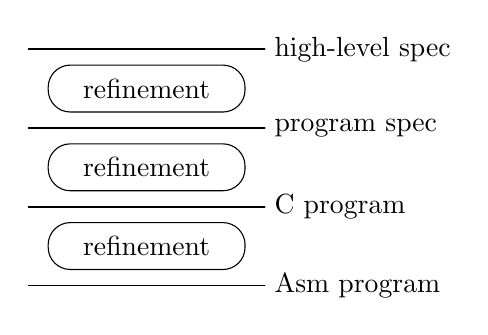
\begin{tikzpicture}[x=1cm,y=1cm,line cap=round]
        % Tunables
        \def\L{3}        % length of the left horizontal lines
        \def\bx{1.5}      % x center of the refinement boxes
        \def\bw{2.5}       % box width (cm)
        \def\bh{0.5}      % box height (cm)
        \def\gap{0.5}      % vertical gap between a line and the box below it

        % Helper macro for one tier: (line_y, label_text)
        \newcommand{\tier}[2]{%
          \draw[line width=0.6pt] (0,#1) -- (\L,#1);
          \node[draw,rounded corners=8pt,minimum width=\bw cm,minimum height=\bh cm,inner sep=5pt]
          at (\bx,#1-\gap) {refinement};
          \node[anchor=west] at (\L,#1) {#2};
        }

        % Tiers
        \tier{3.0}{high-level spec}
        \tier{2.0}{program spec}
        \tier{1.0}{C program}

        % Bottom line + last label (no box below)
        \draw[line width=0.6pt] (0,0) -- (\L,0);
        \node[anchor=west] at (\L,0) {Asm program};
      \end{tikzpicture}
      &
      \begin{tikzpicture}[>=latex]

        % Nodes
        \node[draw,rounded corners=10pt,minimum width=1.5cm,minimum height=2cm] (handler) {handler};
        \node[draw,rounded corners=10pt,minimum width=2cm,minimum height=2cm,right=0.5cm of handler] (refine) {component};
        \node[draw,rounded corners=10pt,minimum width=1.5cm,minimum height=2cm,right=0.5cm of refine] (client) {client};

        % Double arrows between handler and refinement

        \draw[->] ([yshift=0.6cm]handler.east) -- ([yshift=0.6cm]refine.west);
        \draw[<-] ([yshift=0.2cm]handler.east) -- ([yshift=0.2cm]refine.west);
        \draw[->] ([yshift=-0.2cm]handler.east) -- ([yshift=-0.2cm]refine.west);
        \draw[<-] ([yshift=-0.6cm]handler.east) -- ([yshift=-0.6cm]refine.west);

        \draw[->] ([yshift=0.6cm]refine.east) -- ([yshift=0.6cm]client.west);
        \draw[<-] ([yshift=0.2cm]refine.east) -- ([yshift=0.2cm]client.west);
        \draw[->] ([yshift=-0.2cm]refine.east) -- ([yshift=-0.2cm]client.west);
        \draw[<-] ([yshift=-0.6cm]refine.east) -- ([yshift=-0.6cm]client.west);

        % Horizontal lines above and below refinement
        \draw (1,1.3) -- (3.6,1.3);
        \draw (1,-1.3) -- (3.6,-1.3);
        \draw[dashed] (1,1.3) -- (1,-1.3);
        \draw[dashed] (3.6,1.3) -- (3.6,-1.3);

        \node at (1,1.8) {\shortstack[c]{interaction\\[-2pt] convention}};
        \node at (3.6,1.8) {\shortstack[c]{interaction\\[-2pt] convention}};
      \end{tikzpicture}
      \vspace{1.2ex}
      \\
      (a) & (b)
    \end{array}
  \]
  \caption{
    (a) Vertical composition that enables
    transitive composition of refinement properties
    across different abstraction levels.
    (b) Horizontal composition within a single abstraction level.
    The client, component, and handler form a call hierarchy.
  }
  \label{fig:refinement-diagram}
\end{figure}

The core insight underlying this work is that
effective verification frameworks require
\emph{compositionality along multiple dimensions}.
Rather than treating composition as a single concept,
this work recognizes that complex systems require
systematic decomposition along three orthogonal axes.

Compositional semantics provides
a systematic approach to addressing verification challenges
by enabling decomposition along these multiple dimensions.
This multi-dimensional perspective allows
large verification tasks to be broken down
into smaller, independently verifiable components
that can be reliably composed.

Specifically,
compositional semantics acts as
``semantic glue'',
enabling the use of diverse verification methods—such as program logic,
compiler correctness,
type systems,
and manual proofs—within a single cohesive framework.
This allows verification engineers
to select and apply the most suitable tools
for each component,
significantly enhancing verification flexibility and effectiveness.

This framework decomposes verification
along three orthogonal dimensions:

\begin{itemize}
  \item \textbf{Vertical Composition}:
    As illustrated in Fig.~\ref{fig:refinement-diagram}(a),
    vertical composition manages multiple levels of abstraction,
    enabling systems to be verified incrementally
    from high-level specifications down to low-level implementations.
    For example, a high-level functional specification
    can be refined through program specifications to C code,
    and finally to assembly code through compiler correctness.
    Each refinement step is verified independently,
    and the results compose transitively.
  \item \textbf{Horizontal Composition}:
    As shown in Fig.~\ref{fig:refinement-diagram}(b),
    horizontal composition addresses modular reasoning
    within a single abstraction level
    along the \emph{call hierarchy}.
    A component can be invoked by clients
    and can in turn invoke downstream handlers,
    forming a chain of function calls.
    Each component is verified independently
    in a context where it interacts with its environment
    according to specified interaction conventions.
    When verified components adhere to compatible interaction conventions,
    they can be seamlessly composed along this horizontal axis.
  \item \textbf{Spatial Composition}:
    Spatial composition introduces
    a third dimension of compositionality
    by structuring state interactions across different state representations.
    At the lowest level,
    all state is concretized in global memory.
    At higher abstraction levels,
    however, spatial composition allows
    state to be isolated and encapsulated across components,
    with each component responsible for a distinct portion of the state space.
    This enables independent reasoning about disjoint state components—whether
    concrete memory regions, abstract data structures, or logical state predicates—%
    while ensuring that interactions
    occur through disciplined interfaces.
    This explicit management of state boundaries
    strengthens modular reasoning
    and prevents unintended interference.
\end{itemize}

This work develops a
\emph{unified three-dimensional refinement algebra}
that uniformly captures
module composition,
abstraction levels,
and system states.
This algebra enables compositional reasoning
and intuitive graphical representations
through refinement diagrams,
serving as a rigorous foundation
for compositional verification
and supporting clear, intuitive reasoning about complex systems.

\section{Contributions}

\subsubsection{Contribution I: OpenTX and OpenTE Frameworks}

My first main contribution
is the development of the OpenTX and OpenTE frameworks,
which are compositional verification frameworks
based on CompCertO.
OpenTX (Open Transition system with eXternal state)
focuses on layered and spatial composition,
while OpenTE (Open Transition system with Encapsulated state)
further adds state encapsulation capabilities.

The starting point of the framework is the CompCertO's
\emph{open transition system semantics},
a well-established semantic model
explicitly designed to represent interactions
between program components and their environments.
To model interactions among components
and the abstraction levels,
the CompCertO's semantics
has a clear definition of component boundaries,
which naturally aligns with
the three-dimensional algebraic framework.
Moreover,
CompCertO employs \emph{simulation conventions}
to formally establish behavioral refinement relationships
between source- and target-level programs.
These conventions systematically link behaviors
across multiple abstraction levels%
---such as between C source code and
compiled assembly code.

Building upon the CompCertO's open transition systems
and simulation conventions,
this work makes the following extensions
to enhance CompCertO
from a compositional certified compiler
to a compositional verification framework:
\begin{itemize}
  \item Layered Composition:
    this work supplements CompCertO's model of
    translation unit linking
    with a more fundamental layered composition operator.
  \item Spatial Composition:
    this work extends the model
    with a compositional treatment of state,
    allowing both specifications
    and data abstraction
    to act independently
    on different components of the global state.
  \item Memory Separation:
    this work develops a partial commutative monoid structure
    defined on the CompCert memory model
    which bridges the gap between this compositional view
    and the global memory used by CompCert.
  \item State Encapsulation:
    this work extends the model with state encapsulation,
    and explains how the associated primitives
    interact with the model's compositional structure
  \item ClightP Language:
    this work extends the compiler's source language Clight
    to take advantage of the treatment of state.
    The resulting language ClightP
    allows the definition of component-local private variables
    which are kept separate from the global memory.
\end{itemize}

Starting from the CompCertO compiler,
this work extends it with layered composition,
spatial composition,
and memory separation
to obtain the OpenTX framework.
This design is inspired
by the earlier CompCertX work
but surpasses it
by offering a more flexible compositional structure
that fully aligns with the three-dimensional composition principle.
Building on OpenTX,
this work further introduces state encapsulation
and the ClightP semantics
to obtain the OpenTE framework.
These extensions are novel contributions
not found in the existing CompCert literature.
Importantly, all these extensions
are achieved without intrusive modifications
to the original CompCertO semantics,
thanks to the robust foundation
provided by its compositional semantics.

The OpenTE framework
conforms to the three-dimensional algebraic structure,
making it a comprehensive compositional verification framework.
However,
specifications in the OpenTE framework
must be expressed as transition systems,
which primarily emphasize internal transition steps
tailored for compiler correctness verification.
This characteristic limits
the framework's generalizability for broader verification tasks.

\subsubsection{Contribution II: Strategy Model with Refinement Conventions}

My second major contribution
is the development of a
\emph{strategy model}
based on game semantics.

The strategy model serves two key purposes.
First,
it characterizes component behaviors
exclusively through interaction events,
omitting unnecessary internal details
and thereby enabling broader applicability.
Second,
the model is highly flexible and generic,
accounting for various sophisticated reasoning techniques
such as data abstraction and memory separation.
It captures---under a uniform notion of refinement---properties as varied as program correctness results,
the semantics preservation theorem of CompCertO,
the frame property of separation logic,
and representation independence for encapsulated state.

Concretely,
this work highlights the following features
of the strategy model:
\begin{itemize}
  \item Strategy Model:
    this work presents a formalization of the semantics
    that characterizes component behaviors
    as event traces,
    and develops a series of
    composition operators
    to facilitate the definition of components.
  \item Refinement Conventions and Refinement Squares:
    this work extends the idea
    of simulation conventions in CompCertO
    further through \emph{refinement conventions},
    a generalized approach that
    explicitly relates interactions
    across different levels of abstraction.
  \item Embedding CompCertO:
    importantly, CompCertO's semantics
    can be naturally embedded
    within this strategy model,
    enhancing its versatility and integration capability.
\end{itemize}

The theory of game semantics
and its various variants
have been widely studied.
However,
the notion of refinement convention and refinement square
is novel in the context of game semantics.
Furthermore,
to my knowledge,
this is the first mechanized
semantics model based on game semantics
that is capable of
handling real-world verification tasks.

The refinement conventions
and refinement squares
are the key ingredients
to solve Challenge \ref{challenge:abstraction}
by enabling components at different abstraction levels
to be related by the same notion of refinement.
The semantics of the strategy model
captures the interaction of components
as event traces
so that the semantics inherently models
components in open context.
Various composition operators
are developed within the strategy
to make it conform to the three-dimensional algebraic structure
and to accurately represent process interactions.
These efforts effectively solve Challenge \ref{challenge:interaction}.
The strategy model defines component behaviors
through execution traces,
representing the component states entirely
as the interaction histories.
This approach inherently achieves state encapsulation,
directly resolving Challenge \ref{challenge:encapsulation}.
Additionally,
the correctness proofs of
CompCertO's compiler are seamlessly integrated into
the strategy model.
% Furthermore, the strategy model
% itself serves as a suitable semantic specification,
% effectively solving challenge \ref{challenge:specification}.
To resolve the challenge associated with
modeling program loading and execution events,
this work develops a \emph{loader} mechanism
converting CompCertO's open transition systems
into closed, standalone transition systems.
Together, the compiler correctness proofs
and the loader mechanism
effectively solve Challenge \ref{challenge:compilation}.
Lastly, the capability for multi-language reasoning (Challenge \ref{challenge:multi-language}) arises from
leveraging CompCertO's Kripke logical relations.

\subsubsection{Contribution III: Case Studies and Full Mechanization in Rocq}

This work provides a series of case studies
to demonstrate the practicality of the framework.

The first case study concerns
the verification of a bounded queue implementation (Fig.~\ref{fig:bq-code}),
adapted from \citet{rbgs-cal}.
The implementation builds a bounded queue
on top of a ring buffer.
While \citet{rbgs-cal} focused solely
on verifying the high-level specification,
this is extended to an end-to-end result
by verifying CompCertO programs as concrete implementations.
This example also highlights
how state encapsulation enables
a more modular and robust verification approach.

The second case study
examines the verification of programs
shown in Fig.~\ref{fig:readwritehello},
where two components communicate through a pipe:
one encodes a message and writes it to standard output,
while the other reads it from standard input
and decodes it.
This example captures richer patterns of component interaction
and requires mixed-language reasoning,
demonstrating the framework's ability
to handle complex external interactions.

The third case study is
the construction of a CAL instance.
This work has implemented it
using OpenTX, OpenTE, and the strategy model,
respectively.
This staged development demonstrates
how the framework evolves
to support increasingly scalable
and practical verification.
The CAL case study also underscores
how the framework's compositional structures
support generic verification frameworks
instead of ad-hoc verification tasks.

Finally,
the framework is fully mechanized
and validated
within the Rocq proof assistant,
ensuring rigorous, machine-checked proofs.
This mechanization provides practical tools
for verification engineers,
enabling them to conduct
robust and scalable verification efforts confidently.

\section{Structure of the Dissertation}

The remainder of this dissertation is structured as follows:

Chapter \ref{ch:bg} provides the necessary background
on formal verification methodologies,
certified compilation in
CompCert, CompCertO's open semantics,
certified abstraction layers,
and relevant category theory definitions.

Chapter \ref{ch:ox} presents the development of
the OpenTX framework,
introducing layered composition,
state lifting,
and the three-dimensional refinement algebra.
Chapter \ref{ch:oe} explores state encapsulation
and the ClightP language,
further detailing the OpenTE framework's compositional structure.

Chapter \ref{ch:strat} introduces the strategy model,
demonstrating its capabilities
through practical verification examples
and highlighting its balanced abstraction level.
Chapter \ref{ch:rc} elaborates on refinement conventions
and refinement squares,
showcasing how the framework uniformly
captures complex compositional verification scenarios.

Finally,
Chapter \ref{ch:application}
summarizes the applications of the framework
and evaluates its practicality.
Chapter \ref{ch:related}
discusses the related work.
Chapter \ref{ch:conclusion}
concludes the thesis and discusses future work.

%\autoref{ch:conc} concludes the thesis, summarizing the key contributions and discussing future research directions.

Portions of the work presented in this thesis
have previously appeared in peer-reviewed form.
In particular, Chapters \ref{ch:strat} and \ref{ch:rc}
are mostly based on the following publication:

\begin{itemize}
  \item Yu Zhang, Jeremie Koenig, Zhong Shao, and Yuting Wang. ``Unifying Compositional Verification and Certified Compilation with a Three-Dimensional Refinement Algebra.'' In Proceedings of the ACM on Programming Languages (PACMPL), Volume 9, Number POPL, Article 64 (January 2025), 31 pages.
\end{itemize}

This thesis extends and integrates that work with additional material, results, and perspectives.
